\chapter{Simulation Results}
\label{chap:results}

\section{Programming Environment}
\label{sec:environment}

Simulations were carried out using the foam-extend 4.0 fork of the OpenFOAM (Open-Source Field Operation And Manipulation) software project. OpenFOAM was selected as it is a mature and feature rich platform for computational fluid dynamics, and thus already provides many utilities and functionality for tasks such as pre- and post-processing data, run time slection of simulation parameters, and managing very generic mesh structures. It is coded almost entirely in object-oriented C++, making it very flexible for extension, although at over one million lines of code it is still a far from simple endeavour.

The extend fork was chosen over the standard OpenFOAM distribution as it includes an additional density-basesd Navier Stokes (DBNS) solver which implements very closely the basic FVM method which was to be modified. As well, this DBNS library contains several already programmed numerical fluxes and gradient limiters, such that the focus could remain on developing the well-balanced reconstruction without having to code all of the supporting pieces from scratch.


\section{Order Verification Study}
\label{sec:OVS}

An order verification study (OVS) was carried out to verify that the implementation matched the theoretically expected convergence rates.


\section{Toy Problem}
\label{sec:toyProblem}

As previously mentioned, for an initial test of our well-balanced  to the SASI, the simple toy model of FS~\cite{Foglizzo2009,Sato2009} was chosen. The salient details from those papers  are reproduced here. Following the notation of FS, we will denote quantities in the supersonic region before the shock with a subscript `1', in the interior region between the shock and potential step with `in', and in the outflow region past the step with `out'.

A schematic view of the problem domain can be seen in Fig.~\ref{fig:Sato1}, showing how the overall scenario is split into two sub-problems for simulation. The entire test case consists of an supersonic inflow deccelerated at a stationary shock front, followed shortly after by a potential step which further slows the now subsonic flow. This provides a very simplistic analogue to study the mechanisms at play during the inflow, decceleration, and accretion of matter in a collapsing star before supernova.

\begin {figure}
\centering
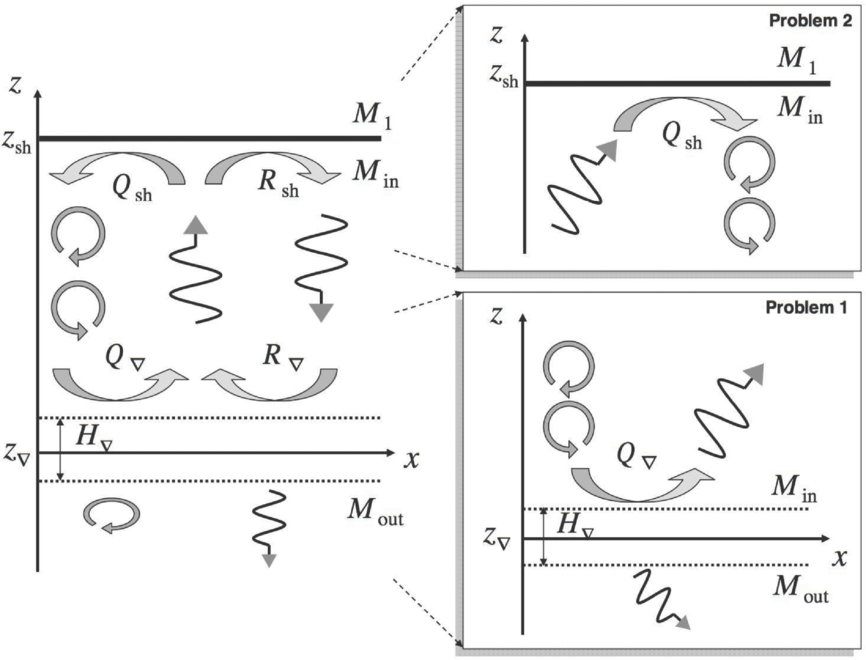
\includegraphics[width=13cm]{figures/Sato1}
\caption {A short caption.}
\label{fig:Sato1}
\end{figure}

For ease of simulation, the potential step and stationary shock are computed separately as sub-problems 1 and 2 respectively. This separation greatly simplifies the introduciton of specific advective and acoustic pertubations to appropriate locations in the interior of the domain, making it much easier to see the interactions of these disturbances at the boundaries (the shock and potential step) between the various flow regions.


\subsection{Sub-Problem 1}

Description of potential step

\subsection{Sub-Problem 2}

Description of the standing shock